\documentclass{article}
\usepackage[headheight=40pt, textheight=560pt]{geometry}
\usepackage{paralist}
\usepackage{scalerel,amssymb}
\usepackage{amsmath}
\usepackage{colortbl}
\usepackage{array}
\usepackage{multirow}
\usepackage{blindtext}
\usepackage{reledmac}
\usepackage{changepage}

\usepackage{pgfplots}
\usepackage{tikz}
\usetikzlibrary{positioning}
\usetikzlibrary{shapes.geometric, arrows}
\tikzstyle{arrow} = [thick,->,>=stealth]

\usepackage{graphicx}
\usepackage{stix}

\newcommand{\tableflip}{$($\rotatebox{45}{$\smile$}$^{\circ}\smwhtsquare^{\circ})\rotatebox{45}{$\smile$}\mkern-6mu\frown$\raisebox{0.5ex}{$\bot$}$\mkern-3.5mu-\mkern-3.5mu$\raisebox{0.5ex}{$\bot$}}

\usepackage{stackengine}
\def\apeqA{\SavedStyle\sim}
\def\apeq{\setstackgap{L}{\dimexpr.5pt+1.5\LMpt}\ensurestackMath{%
  \ThisStyle{\mathrel{\Centerstack{{\apeqA} {\apeqA} {\apeqA}}}}}}

\usepackage{fancyhdr}
\fancyhead[L]{
	\begin{tabular}{ll}
		\begin{tabular}{l}
			\includegraphics[scale=0.13]{distributed}
		\end{tabular}	
		&
		\begin{tabular}{l}
			\LARGE \textbf{Distributed Algorithms} \\
			\Large \textsc{Lectures}
		\end{tabular}
	\end{tabular}
}
\fancyhead[R]{
	\begin{tabular}{r}
		16-124-836 \\
		Marcel \textsc{Zauder}
	\end{tabular}
}
\renewcommand{\headrulewidth}{0.4pt}
\fancyfoot[C]{\thepage}
\renewcommand{\footrulewidth}{0.4pt}

\usepackage{hyperref}

\begin{document}
	\pagestyle{fancy}
	\section{Introduction - February 19, 2020}
	\begin{adjustwidth}{2em}{2em}
		\subsection{Defining Dependable Systems}
		\begin{adjustwidth}{2em}{2em}
			\textsc{Quotes:}
			\begin{adjustwidth}{2em}{}
				\textit{A distributed system is a system where a computer of which you did not know it exists can prevent you from getiing your job done.} - Leslie \textsc{Lamport}
			\end{adjustwidth}
			\vspace{0.2cm}
			\begin{adjustwidth}{2em}{}
				\textit{There is perhaps a market for maybe five computers in the world.} - TJ \textsc{Watson}
			\end{adjustwidth}
			\hfill \\
			\textsc{Fault} $\rightarrow$ \textsc{Error} $\rightarrow$ \textsc{Failure}
			\begin{compactenum}[-]
				\item Train delayed because of tree has fallen on the tracks
				\item Travelers reach destination too late
				\item Alice misses her exam
			\end{compactenum}
			\vspace{0.2cm}
			\begin{tabular}{|l|lll|}
				\hline
				& \underline{\textsc{Fault}} & \underline{\textsc{Error}} & \underline{\textsc{Failure}} \\
				\hline
				Train: & Tree fallen & no train & delay for passengers \\
				Journey: & Train delay & delay & reached destination 2h after intention \\
				Exam: & arrival 2h late & missed time-slot & repeat exam \\
				\hline
			\end{tabular}
			\hfill \\
			\underline{\textsc{Fault:}} cause of failure \\
			\underline{\textsc{Error:}} internal state of system, not according to specification \\
			\underline{\textsc{Failure:}} observable deviation of specification
			\hfill \\ \\
			\underline{\textsc{Fault} examples:}
			\begin{compactenum}[-]
				\item timing
				\item cables
				\item power supply
				\item messages lost
				\item data loss (solved with RAIDs)
			\end{compactenum}
			\subsubsection{\underline{How to make systems tolerate faults}}
			\begin{adjustwidth}{2em}{}
				\begin{compactenum}[-]
					\item \textsc{Prevention}
					\item \textsc{Tolerance}
					\begin{compactenum}[\textbullet]
						\item Replication/Redundancy
						\item Recovery
					\end{compactenum}
					\item \textsc{Removal}
					\item \textsc{Forecasting/Prediction}
				\end{compactenum}
			\end{adjustwidth}
			\hfill \\
			\textsc{Safety} $\neq$ \textsc{Security} \\
			\textsc{Safety} is connected to loss of live/material due to accidents \\
			\textsc{Security} is connected to malicious intent
			\subsubsection{Defining distributed computation}
			\begin{adjustwidth}{2em}{}
				Processes $\Pi = \{ p,q,r,s \ldots \}$ \\
				$\mid \Pi \mid = N$
				
				\begin{adjustwidth}{1em}{}
					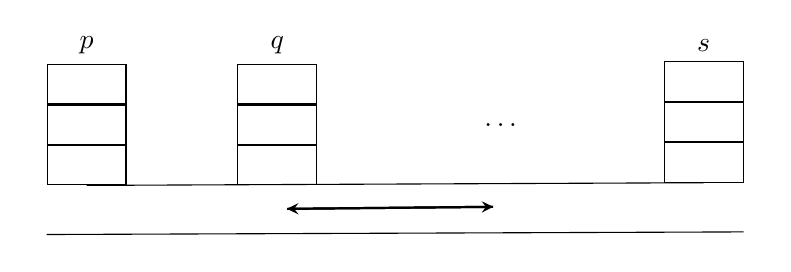
\begin{tikzpicture}
						\coordinate (start);
							
						%Nodes
						\node [right=of start] (p) {$p$};
						\node (rect) [draw,thin,minimum width=1cm,minimum height=0.5cm, below=0cm of p] (1stp) {};
						\node (rect) [draw,thin,minimum width=1cm,minimum height=0.5cm, below=0cm of 1stp] (2ndp) {};
						\node (rect) [draw,thin,minimum width=1cm,minimum height=0.5cm, below=0cm of 2ndp] (3rdp) {};
						
						\node [right=2cm of p] (q) {$q$};
						\node (rect) [draw,thin,minimum width=1cm,minimum height=0.5cm, below=0cm of q] (1stq) {};
						\node (rect) [draw,thin,minimum width=1cm,minimum height=0.5cm, below=0cm of 1stq] (2ndq) {};
						\node (rect) [draw,thin,minimum width=1cm,minimum height=0.5cm, below=0cm of 2ndq] (3rdq) {};
						
						\node [right=2cm of 2ndq] (ldots) {\ldots};
						
						\node [right=5cm of q] (s) {$s$};
						\node (rect) [draw,thin,minimum width=1cm,minimum height=0.5cm, below=0cm of s] (1sts) {};
						\node (rect) [draw,thin,minimum width=1cm,minimum height=0.5cm, below=0cm of 1sts] (2nds) {};
						\node (rect) [draw,thin,minimum width=1cm,minimum height=0.5cm, below=0cm of 2nds] (3rds) {};
						
						\node [below left=0.5cm and 0cm of 3rdp] (pbelow) {};	
						\node [below right=0.5cm and 0cm of 3rds] (sbelow) {};	
						\node [below =0.175cm of 3rdq] (qbelow) {};	
						\node [below =0.775cm of ldots] (ldotsbelow) {};	
						
						%Lines
						\draw (3rdp.south) -- (3rds.south);
						\draw (pbelow) -- (sbelow);
						\draw[arrow] (qbelow) -- (ldotsbelow);
						\draw[arrow] (ldotsbelow) -- (qbelow);
							
						%Lines
						%\draw[arrow] (start) -- node[ anchor=south ]{$m$} (Enc.west);
						%\draw[arrow] (Enc.east) -- node[ anchor=south ]{$c$} (Dec.west);
						%\draw[arrow] (Enc.east) -| (Eve.north);
						%\draw[arrow] (Dec.east) -- node[ anchor=south ]{$m'$} (stop.west);
							
					\end{tikzpicture}
				\end{adjustwidth}
				\hfill \\
				\underline{\textsc{Components}} \\
				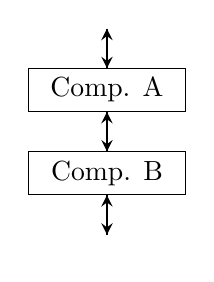
\begin{tikzpicture}					
					\coordinate (start);
					
					%Nodes
					\node (rect) [draw,thin,minimum width=2cm,minimum height=0.5cm, below=0.5cm of start] (CompA) {Comp. A};
					\node (rect) [draw,thin,minimum width=2cm,minimum height=0.5cm, below=0.5cm of CompA] (CompB) {Comp. B};
					\node [below=0.5cm of CompB] (stop) {};
					
					%Lines
					\draw[arrow] (start) -- (CompA.north);
					\draw[arrow] (CompA.north) -- (start);
					\draw[arrow] (CompA.south) -- (CompB.north);
					\draw[arrow] (CompB.north) -- (CompA.south);
					\draw[arrow] (stop) -- (CompB.south);
					\draw[arrow] (CompB.south) -- (stop);
				\end{tikzpicture}
				\hfill \\
				\textsc{Events} for Component $c$:
				\[
					\langle c, event \mid param_1 , param_2 \ldots \rangle
				\]
				\underline{upon} $\langle c, ev_1 \mid param_1 \rangle$ \underline{do}
				\begin{adjustwidth}{1em}{}
					do something \\
					\underline{trigger} $\langle \textit{b, domore} \mid p \rangle$
				\end{adjustwidth}
				\hfill \\
				\underline{upon} $\langle \textit{b, domore} \mid p \rangle$ \underline{do}
			\end{adjustwidth}
			\subsubsection{Layered modules}
			\begin{adjustwidth}{2em}{}
				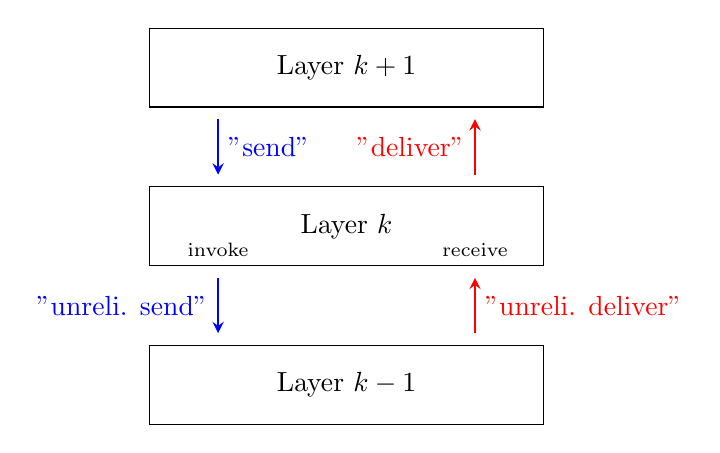
\begin{tikzpicture}
					\coordinate (start);
					
					%Nodes
					\node (rect) [draw,thin,minimum width=5cm,minimum height=1cm] (Layerk+1) {Layer $k+1$};
					\node (rect) [draw,thin,minimum width=5cm,minimum height=1cm, below=1cm of Layerk+1] (Layerk) {Layer $k$};
					\node (rect) [draw,thin,minimum width=5cm,minimum height=1cm, below=1cm of Layerk] (Layerk-1) {Layer $k-1$};
					
					\node [below left = -0.1cm and -1cm of Layerk+1] (sendOut) {};
					\node [below right = -0.1cm and -1cm of Layerk+1] (deliverIn) {};
					\node [above left = -0.1cm and -1cm of Layerk] (sendIn) {};
					\node [above right = -0.1cm and -1cm of Layerk] (deliverOut) {};
					\node [below left = -0.1cm and -1cm of Layerk] (unSendOut) {};
					\node [below right = -0.1cm and -1cm of Layerk] (unDeliverIn) {};
					\node [above left = -0.1cm and -1cm of Layerk-1] (unSendIn) {};
					\node [above right = -0.1cm and -1cm of Layerk-1] (unDeliverOut) {};
					
					\node [above=-0.1cm of unSendOut] (invoke) {\scriptsize invoke};
					\node [above=-0.1cm of unDeliverIn] (receive) {\scriptsize receive};
					
					%Lines
					\draw[blue, arrow] (sendOut) -- node[ anchor=west ]{"send"} (sendIn);
					\draw[red, arrow] (deliverOut) -- node[ anchor=east ]{"deliver"} (deliverIn);
					\draw[blue, arrow] (unSendOut) -- node[ anchor=east ]{"unreli. send"} (unSendIn);
					\draw[red, arrow] (unDeliverOut) -- node[ anchor=west ]{"unreli. deliver"} (unDeliverIn);
				\end{tikzpicture}
				\hfill \\
				Events either travel:
				\begin{compactenum}[-]
					\item upwards (red): indication
					\item downwards (blue): request
				\end{compactenum}
				\vspace{0.3cm}
				Events on a given layer may be:
				\begin{compactenum}[-]
					\item input events (IN)
					\item output events (OUT)
				\end{compactenum}
			\end{adjustwidth}
			\subsubsection{Module Jobhandler}
			\begin{adjustwidth}{2em}{}
				\underline{Events:}
				\begin{adjustwidth}{1em}{}
					Request: $\langle \textit{jh, handle} \mid \textit{job} \rangle$ \\
					Indication: $\langle \textit{jh, confirm} \mid \textit{job} \rangle$
				\end{adjustwidth}
				\underline{Properties:}
				\begin{adjustwidth}{1em}{}
					Every job submitted for handling is eventually confirmed.
				\end{adjustwidth}
				\hfill \\
				\underline{Implementation (synchronized)} \textsc{JobHandler} \\
				\underline{State}
				\begin{adjustwidth}{1em}{}
					\ldots
				\end{adjustwidth}
				\underline{upon} $\langle \textit{jh, handle} \mid \textit{job} \rangle$ \underline{do}
				\begin{adjustwidth}{1em}{}
					"process job" \\
					\underline{trigger} $\langle \textit{jh, confirm} \mid \textit{job} \rangle$
				\end{adjustwidth}
				\vspace{0.2cm}
				\underline{upon} \ldots \\
				\underline{upon} \ldots \\ \\
				\underline{Implementation (asynchronized)} \textsc{JobHandler} \\
				\underline{State}
				\begin{adjustwidth}{1em}{}
					\textit{buf} $\leftarrow \emptyset$
				\end{adjustwidth}
				\underline{upon} $\langle \textit{jh, handle} \mid \textit{job} \rangle$ \underline{do}
				\begin{adjustwidth}{1em}{}
					\textit{buf} $\leftarrow$ \textit{buf} $\cup \{ \textit{job} \}$ \\
					\underline{trigger} $\langle \textit{jh, confirm} \mid \textit{job} \rangle$
				\end{adjustwidth}
				\vspace{0.2cm}
				\underline{upon} \textit{buf} $\neq \emptyset$ \underline{do}
				\begin{adjustwidth}{1em}{}
					\textit{job} $\leftarrow$ some element of \textit{buf} \\
					"process job" \\
					\textit{buf} $\leftarrow$ \textit{buf} $\setminus \{ \textit{job} \}$
				\end{adjustwidth}
			\end{adjustwidth}
		\end{adjustwidth}
		\subsection{Concurrency and Replication in Distributed Systems}
		\begin{adjustwidth}{2em}{2em}
		\end{adjustwidth}
	\end{adjustwidth}
	
	\newpage
	
	\section{Models and Abstructions - February 26, 2020}
	\begin{adjustwidth}{2em}{2em}		
		\subsection{Processes and Protocols}
		\begin{adjustwidth}{2em}{2em}
			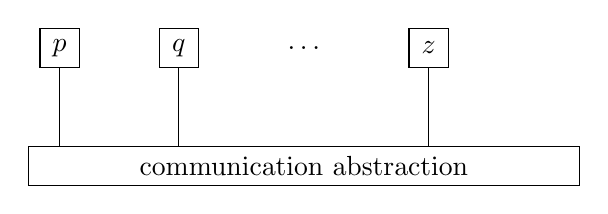
\begin{tikzpicture}
				\coordinate (start);
							
				%Nodes
				\node (rect) [draw,thin,minimum width=0.5cm,minimum height=0.5cm] (p) {$p$};
				\node (rect) [draw,thin,minimum width=0.5cm,minimum height=0.5cm, right=1cm of p] (q) {$q$};
				\node [right=1cm of q] (ldots) {$\ldots$};
				\node (rect) [draw,thin,minimum width=0.5cm,minimum height=0.5cm, right=1cm of ldots] (z) {$z$};
				
				\node (rect) [draw,thin,minimum width=7cm,minimum height=0.5cm, below=1.1cm of ldots] {communication abstraction};
				
				\node [below=1cm of p] (bp) {};
				\node [below=1cm of q] (bq) {};
				\node [below=1cm of z] (bz) {};
				
				%Lines
				\draw (p) -- (bp);
				\draw (q) -- (bq);
				\draw (z) -- (bz);
				
			\end{tikzpicture}
			\begin{enumerate}[-]
				\item Set of Processes $\Pi$ \\
				$\mid \Pi \mid = N$
				\item A process is an automaton
				\item A protocol is a set of processes
			\end{enumerate}
			\subsubsection{Execution}
			\begin{adjustwidth}{2em}{}
				\begin{enumerate}[-]
					\item Each computation step and every step of sending a message or receiving a message is an event
					\item An execution (history) is a sequence of all events of the processes as seen by a (hypothetical) global observer
					\item trace = execution
				\end{enumerate}
			\end{adjustwidth}
			\subsubsection{Properties}
			\begin{adjustwidth}{2em}{}
				Used for specifying the abstractions: \\
				\begin{enumerate}[\footnotesize{\textbullet}]
					\item \textbf{Safety properties} (\textit{something "bad" has not happened}) \\
					If a property $P$ has been violated in some execution $E$, then there exists a prefix $E'$ of $E$ such that in every extension of $E'$, property $P$ is violated
					\item \textbf{Liveness properties} (\textit{something "good" will happen in the future} [\textsc{eventually}]) \\
					Property $P$ can be satisfied by some extension $\stackrel{\sim}{E}$ of a given execution $E$
				\end{enumerate}
				\hfill \\
				\textit{Safety} or \textit{Liveness} alone is not very useful. Only combination of both properties.
			\end{adjustwidth}
			\subsubsection{Process Failures}
			\begin{adjustwidth}{2em}{}
				A process consists of different modules - if one of them fails the entire thing fails at once.
				\begin{enumerate}[-]
					\item[$\bigstar$] \underline{\textit{\textbf{Crashes}}}
					\item \textit{Omission failures }(\textit{message sending and receiving events are omitted})
					\item \textit{Crash-Recovery Failure}
					\begin{enumerate}[\tiny{\textbullet}]
						\item store(-) operation to write to stable storage
						\item upon recovery, one can restore(-) data from this stable storage
					\end{enumerate}
					\item \textit{Eavesdropping Fault}
					\item[$\bigstar$] \underline{\textit{\textbf{Arbitrary Fault (Byzantine Fault)}}}
				\end{enumerate}
			\end{adjustwidth}
		\end{adjustwidth}
		\subsection{Cryptographic Abstraction}
		\begin{adjustwidth}{2em}{2em}
			\begin{enumerate}[\footnotesize{\textbullet}]
				\item \textbf{\textit{Hash functions}} (SHA-256) \\
				$H:{ 0,1 } ^{\star} \rightarrow \{ 0,1 \} ^{k}$
				\begin{enumerate}[-]
					\item collision-free: difficult to find $x, x'$ with $x \neq x'$ and $H(x) = H(x')$
				\end{enumerate}
				\item \textbf{\textit{Message-Authentication-Code (MAC)}} (HMAC-SHA256)
				\begin{enumerate}[-]
					\item $\textit{authentication}(p, q, m) \rightarrow a$
					\item $\textit{verifyAuth}(p, q, m, a) \rightarrow$ \textsc{Yes/No}
				\end{enumerate}
				\item \textbf{\textit{Digital Signatures}} (RSA, (EC)DSA)
				\begin{enumerate}[-]
					\item $\textit{sign}(p, m) \rightarrow s$
					\item $\textit{verifySign}(p,m,s) \rightarrow$ \textsc{Yes/No}
					\item[$\bigstar$] \underline{\textit{Correctness}}: \\
					$\forall m,p: \ \textit{verifySign}(p, m, \textit{sign}(p,m)) \ =$ \textsc{Yes}
					\item[$\bigstar$] \underline{\textit{Security}}: \\
					$\forall m, p, s: \ \textit{verifySign}(p, m, s) \ =$ \textsc{No}, unless $p$ has executed $sign(p,m) \rightarrow s$
				\end{enumerate}
			\end{enumerate}
		\end{adjustwidth}
		\subsection{Communication Abstraction}
		\begin{adjustwidth}{2em}{2em}
			Every process can send messages to every other process.
			\subsubsection{Stubborn point-to-point links}
			\begin{adjustwidth}{2em}{}
				\textbf{\underline{Events:}}
				\begin{enumerate}[]
					\item $\langle sl.send \mid q,m \rangle$ \{ \textit{send message $m$ to process $q$}
					\item $\langle sl.deliver \mid p,m \rangle$ \{ deliver a received message $m$ from process $p$ 
				\end{enumerate}
				\textbf{\underline{Properties:}}
				\begin{enumerate}[]
					\item \underline{\textit{Stubborn delivery}:} \\
					If a process sends a message $m$ to process $q$, then $m$ is infinitely often delivered at $q$.
					\item \underline{\textit{No creation}:} \\
					If some process $q$ delivers some message $m$ from $p$ then process $p$ has previously sent $m$ to $q$.
				\end{enumerate}
			\end{adjustwidth}
			\subsubsection{Perfect point-to-point links}
			\begin{adjustwidth}{2em}{}
				\textbf{\underline{Events:}}
				\begin{enumerate}[]
					\item $\langle sl.send \mid q,m \rangle$
					\item $\langle sl.deliver \mid p,m \rangle$
				\end{enumerate}
				\textbf{\underline{Properties:}}
				\begin{enumerate}[]
					\item \underline{\textit{Reliable delivery}:} \\
					If a correct process sends a message $m$ to a correct process $q$ then $q$ eventually delivers $m$
					\item \underline{\textit{No creation}:} \\
					If process $q$ delivers some $m$ from process $p$ then $p$ has sent $m$ to $q$
					\item \underline{\textit{At-most-once delivery:}} \\
					Every message $m$ is delivered at most once from $p$ to $q$.
				\end{enumerate}
			\end{adjustwidth}
			\subsubsection{Alg. impl. perfect links (pl) from stubborn links (sl)}
			\begin{adjustwidth}{2em}{}
				\underline{\textsc{Init:}} \\
				$\mathbb{D} \leftarrow \emptyset$ \\
				\underline{upon} $\langle pl.send \mid q,m \rangle$ \underline{do}
				\begin{adjustwidth}{1em}{}
					trigger $\langle sl,send \mid q,m \rangle$ \\
					\underline{upon} $\langle sl.deliver \mid p,m \rangle$ \underline{do}
					\begin{adjustwidth}{1em}{}
						\underline{if} $(p,m) \not\in \mathbb{D}$ \underline{then}
						\begin{adjustwidth}{1em}{}
							$\mathbb{D} \leftarrow \mathbb{D} \cup \{ (p,m) \}$ \\
							trigger $\langle pl.deliver \mid p,m \rangle$ \\
							\ldots
						\end{adjustwidth}
					\end{adjustwidth}
				\end{adjustwidth}
			\end{adjustwidth}
		\end{adjustwidth}
		\subsection{Timing Assumptions}
		\begin{adjustwidth}{2em}{2em}
			\begin{enumerate}[\footnotesize{\textbullet}]
				\item \underline{\textbf{Asynchronous model} (\textit{Logical Timing})}
				\begin{enumerate}[-]
					\item \textbf{\textit{One Process}} \\
					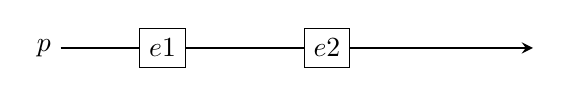
\begin{tikzpicture}
						%Nodes
						\node (rect) (p) {$p$};
						\node [right=6cm of p] (end) {};
					
						%Lines
						\draw[arrow] (p) -- (end);
					
						\node (rect) [draw,thin,fill=white,minimum width=0.5cm,minimum height=0.5cm, right=1cm of p] (e1) {$e1$};
						\node (rect) [draw,thin,fill=white,minimum width=0.5cm,minimum height=0.5cm, right=1.5cm of e1] (e2) {$e2$};
					\end{tikzpicture} \\
					If $e2$ happened after $e1$ in one process, we know the sequence of events.
					\item \textbf{\textit{Two Processes}} \\
					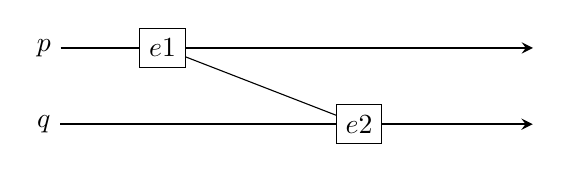
\begin{tikzpicture}
						%Nodes
						\node (rect) (p) {$p$};
						\node [right=6cm of p] (endp) {};
						
						\node (rect) [below=0.5cm of p] (q) {$q$};
						\node [right=6cm of q] (endq) {};
					
						%Lines
						\draw[arrow] (p) -- (endp);
						\draw[arrow] (q) -- (endq);
					
						\node (rect) [draw,thin,fill=white,minimum width=0.5cm,minimum height=0.5cm, right=1cm of p] (e1) {$e1$};
						\node (rect) [draw,thin,fill=white,minimum width=0.5cm,minimum height=0.5cm, right=3.5cm of q] (e2) {$e2$};
						
						\draw (e1) -- (e2);
					\end{tikzpicture} \\
					If we know that $e1$ caused $e2$, we know that $e2$ happened after $e1$.
					\item \textbf{\textit{Three processes}} \\
					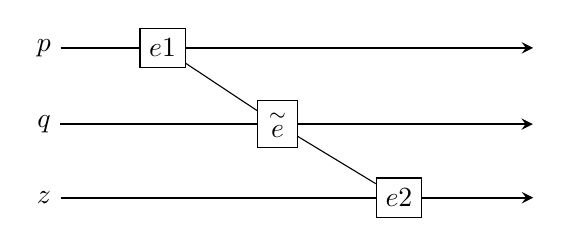
\begin{tikzpicture}
						%Nodes
						\node (rect) (p) {$p$};
						\node [right=6cm of p] (endp) {};
						
						\node (rect) [below=0.5cm of p] (q) {$q$};
						\node [right=6cm of q] (endq) {};
						
						\node (rect) [below=0.5cm of q] (z) {$z$};
						\node [right=6cm of z] (endz) {};
					
						%Lines
						\draw[arrow] (p) -- (endp);
						\draw[arrow] (q) -- (endq);
						\draw[arrow] (z) -- (endz);
					
						\node (rect) [draw,thin,fill=white,minimum width=0.5cm,minimum height=0.5cm, right=1cm of p] (e1) {$e1$};
						\node (rect) [draw,thin,fill=white,minimum width=0.5cm,minimum height=0.5cm, right=2.5cm of q] (et) {$\stackrel{\sim}{e}$};
						\node (rect) [draw,thin,fill=white,minimum width=0.5cm,minimum height=0.5cm, right=4cm of z] (e2) {$e2$};
						
						\draw (e1) -- (et);
						\draw (et) -- (e2);
					\end{tikzpicture} \\
					Transitivity holds across processes, so if $e1$ caused $\stackrel{\sim}{e}$ which cause $e2$, $e2$ happened after $e1$.
				\end{enumerate}
				\item Other time models exist
			\end{enumerate}
		\end{adjustwidth}
	\end{adjustwidth}
	
	\newpage
	
	\section{3rd Lecture - \today}
	\begin{adjustwidth}{2em}{2em}
		\subsection{sub}
		\begin{adjustwidth}{2em}{2em}
		\end{adjustwidth}
	\end{adjustwidth}
\end{document}